\subsubsection{Kettenmatrix}\label{subsec:kettenmatrix}

Die ABCD-Matrix ist eine weitere gängige Variante, um das Verhalten von 2-Toren zu beschreiben. Diese Variante hat den Vorteil, dass man in Serie geschaltene 2-Tore ohne grossen Aufwand zusammen rechnen kann. Sobald man die einzelnen ABCD-Matrixen gebildet hat und die Schaltung soweit vereinfacht ist, dass nur noch in Serie geschaltene ABCD-Matrixen vorzufinden sind, können diese miteinander multipliziert werden. Das Matrix-Produkt stellt dann die ABCD-Matrix der Gesamtschaltung dar. Folgende gängigen Schaltungen helfen die ABCD-Matrixen der einzelnen Schaltungsteilen zu bilden.

Die Längsimpedanz lässt sich anhand der ABCD-Matrix A\textsubscript{L} (Formel \ref{equ:horizImpedance}) darstellen
\begin{figure}[H]
	\begin{minipage}[h]{0.45\linewidth}
		\centering
		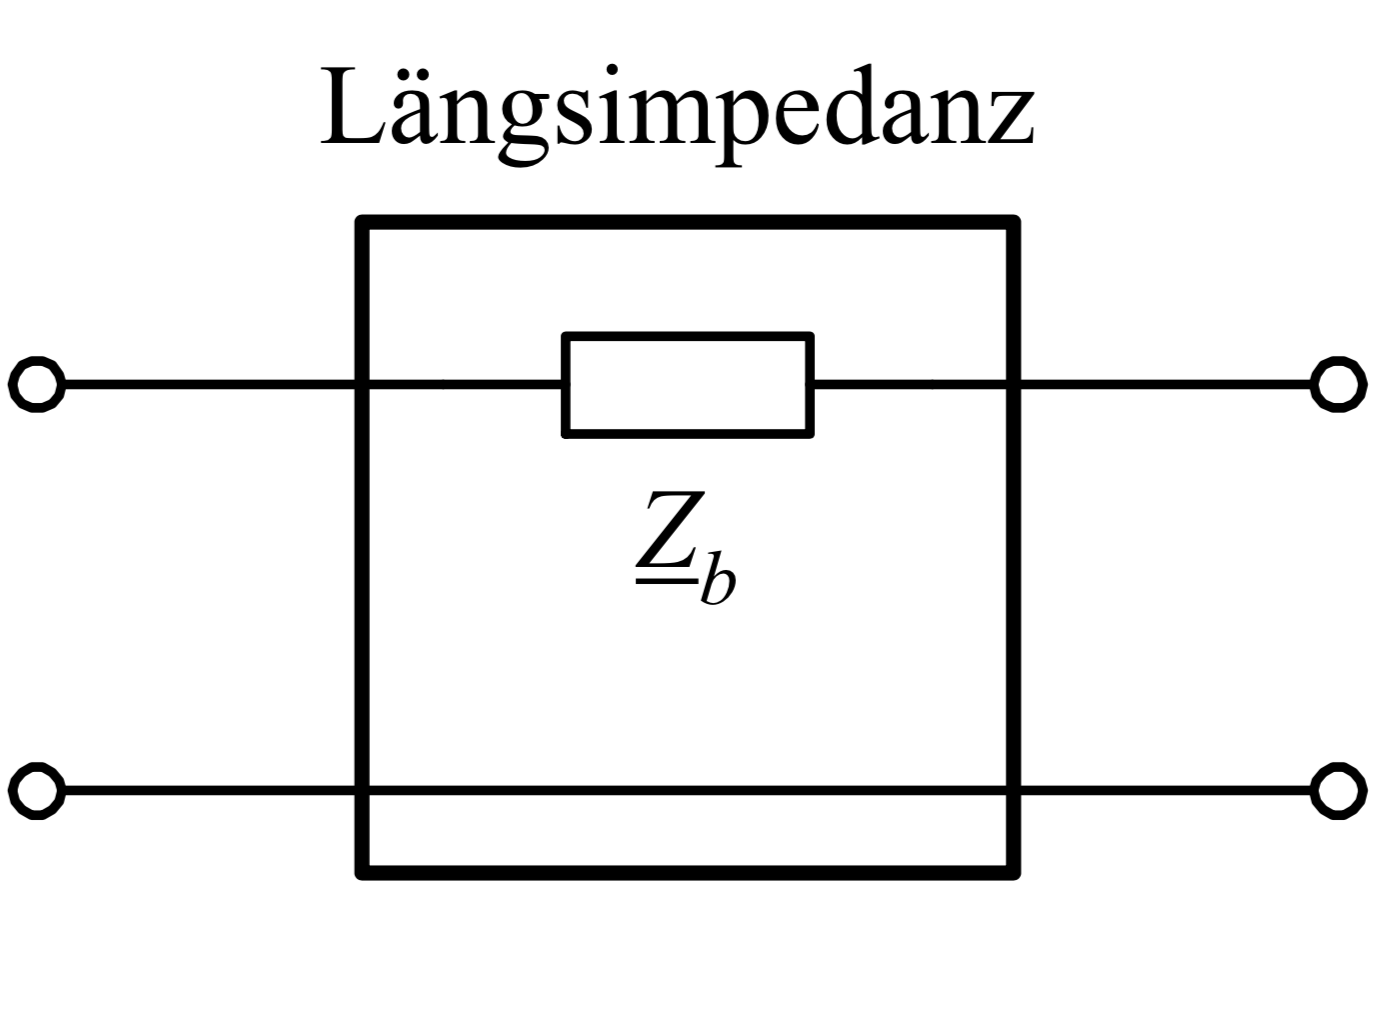
\includegraphics[width = 3cm]{h_impedance.png}
		\caption{Längsimpedanz \cite{2torTabelle}}
	\end{minipage}
	\begin{minipage}[h]{0.45\linewidth}
		\centering
		\begin{equation}\label{equ:horizImpedance}
			A_L = \left[\begin{matrix}
			1&\underline{Z}_b\\0&1
			\end{matrix}\right]
		\end{equation}
	\end{minipage}
\end{figure}
Die Querimpedanz lässt sich anhand der ABCD-Matrix A\textsubscript{Q} (Formel \ref{equ:verticImpedance}) darstellen
\begin{figure}[H]
	\begin{minipage}[h]{0.45\linewidth}
		\centering
		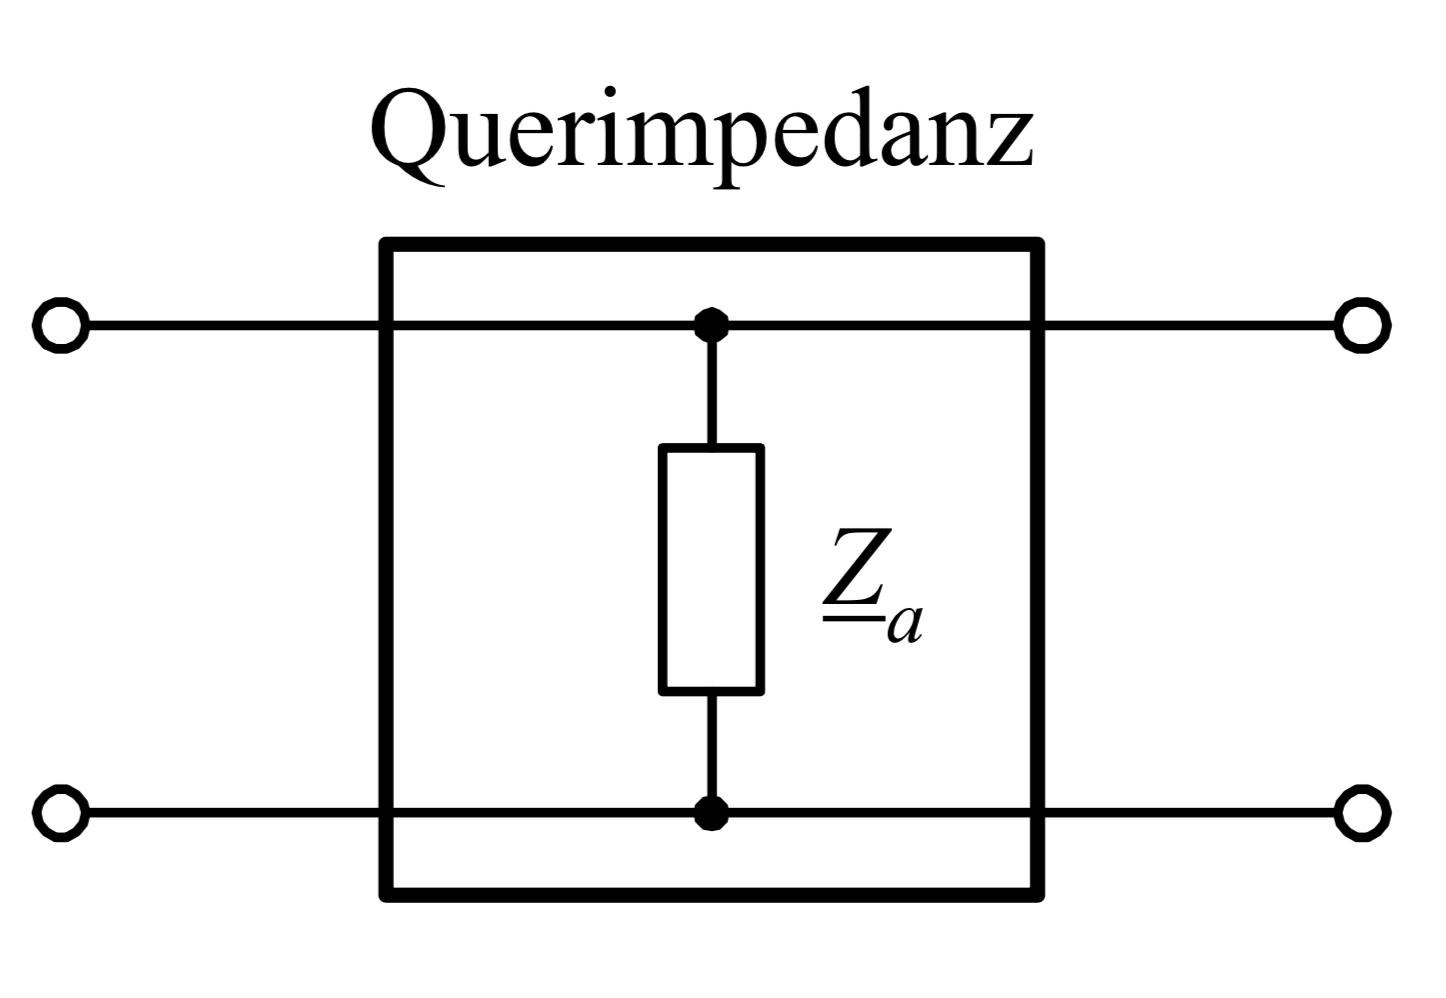
\includegraphics[width = 3cm]{v_impedance.png}
		\caption{Querimpedanz \cite{2torTabelle}}
	\end{minipage}
	\begin{minipage}[h]{0.45\linewidth}
		\centering
		\begin{equation}\label{equ:verticImpedance}
			A_Q = \left[\begin{matrix}
			1&0\\\frac{1}{\underline{Z}_a}&1
			\end{matrix}\right]
		\end{equation}
	\end{minipage}
\end{figure}
Die Impedanz eines T-Glieds lässt sich anhand der ABCD-Matrix $A_T$ (Formel \ref{equ:tImpedance}) darstellen
\begin{figure}[H]
	\begin{minipage}[h]{0.45\linewidth}
		\centering
		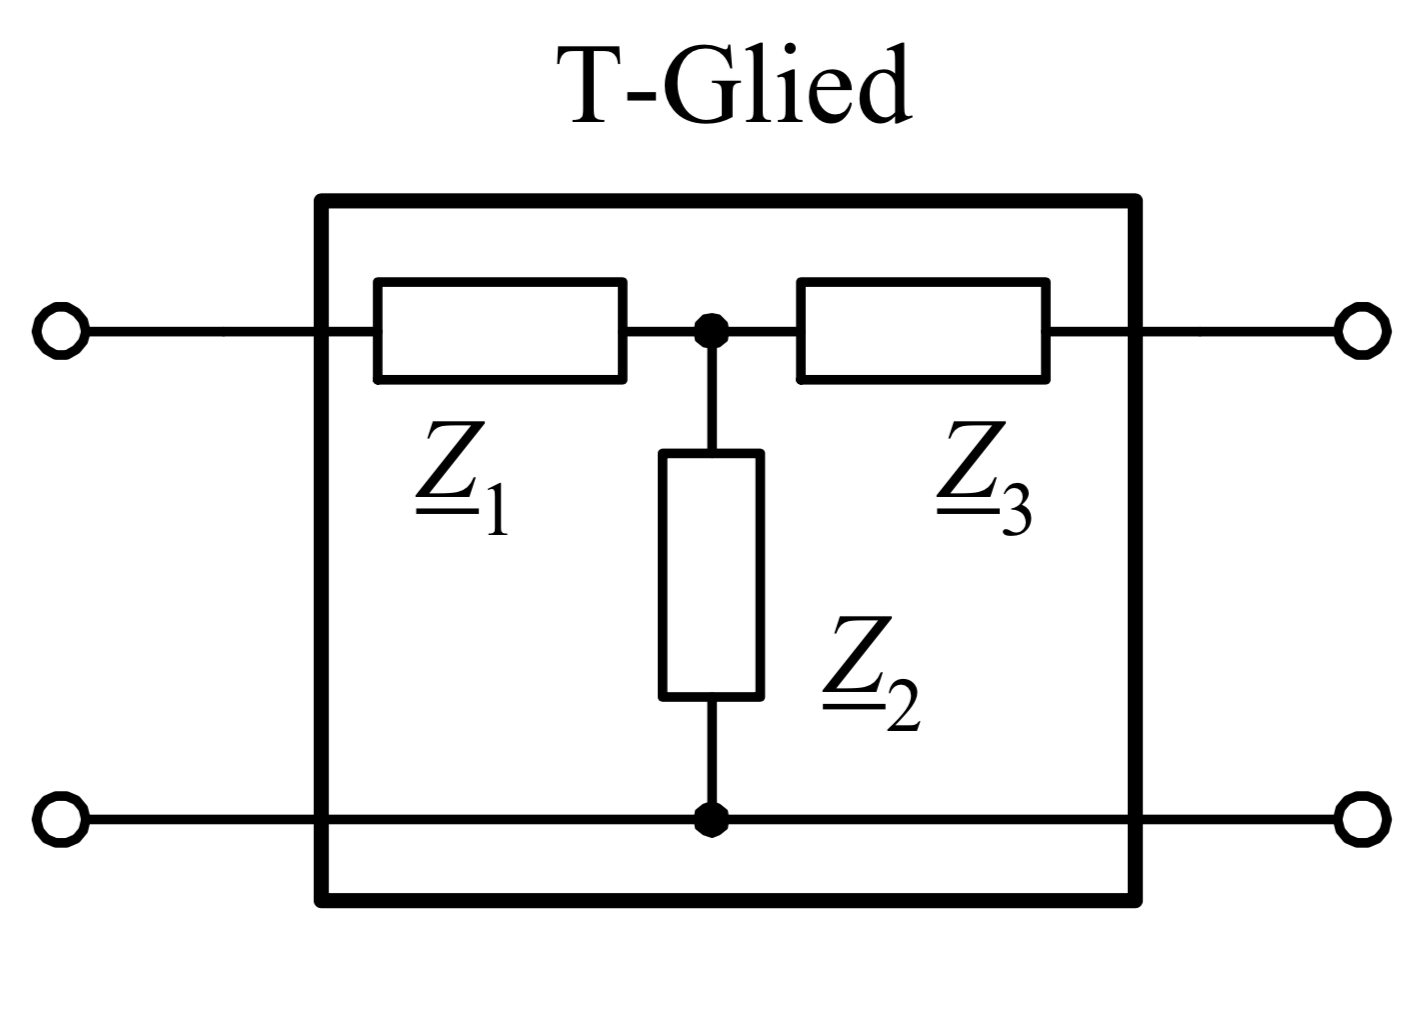
\includegraphics[width = 3cm]{t_impedance.png}\label{fig:tImpedance}
		\caption{T-Glied \cite{2torTabelle}}
	\end{minipage}
	\begin{minipage}[h]{0.45\linewidth}
		\centering
		\begin{equation}\label{equ:tImpedance}
			A_T = \left[\begin{matrix}
			1+\frac{\underline{Z}_2}{\underline{Z}_3}&\underline{Z}_1+\underline{Z}_3+\frac{\underline{Z}_1\underline{Z}_3}{\underline{Z}_2}\\
			\frac{1}{\underline{Z}_2}&1+\frac{\underline{Z}_3}{\underline{Z}_2}
			\end{matrix}\right]
		\end{equation}
	\end{minipage}
\end{figure}
Die Impedanz eines  $\pi$-Glieds lässt sich anhand der ABCD-Matrix $A_\pi$ (Formel \ref{equ:piImpedance}) darstellen
\begin{figure}[H]
	\begin{minipage}[h]{0.45\linewidth}
		\centering
		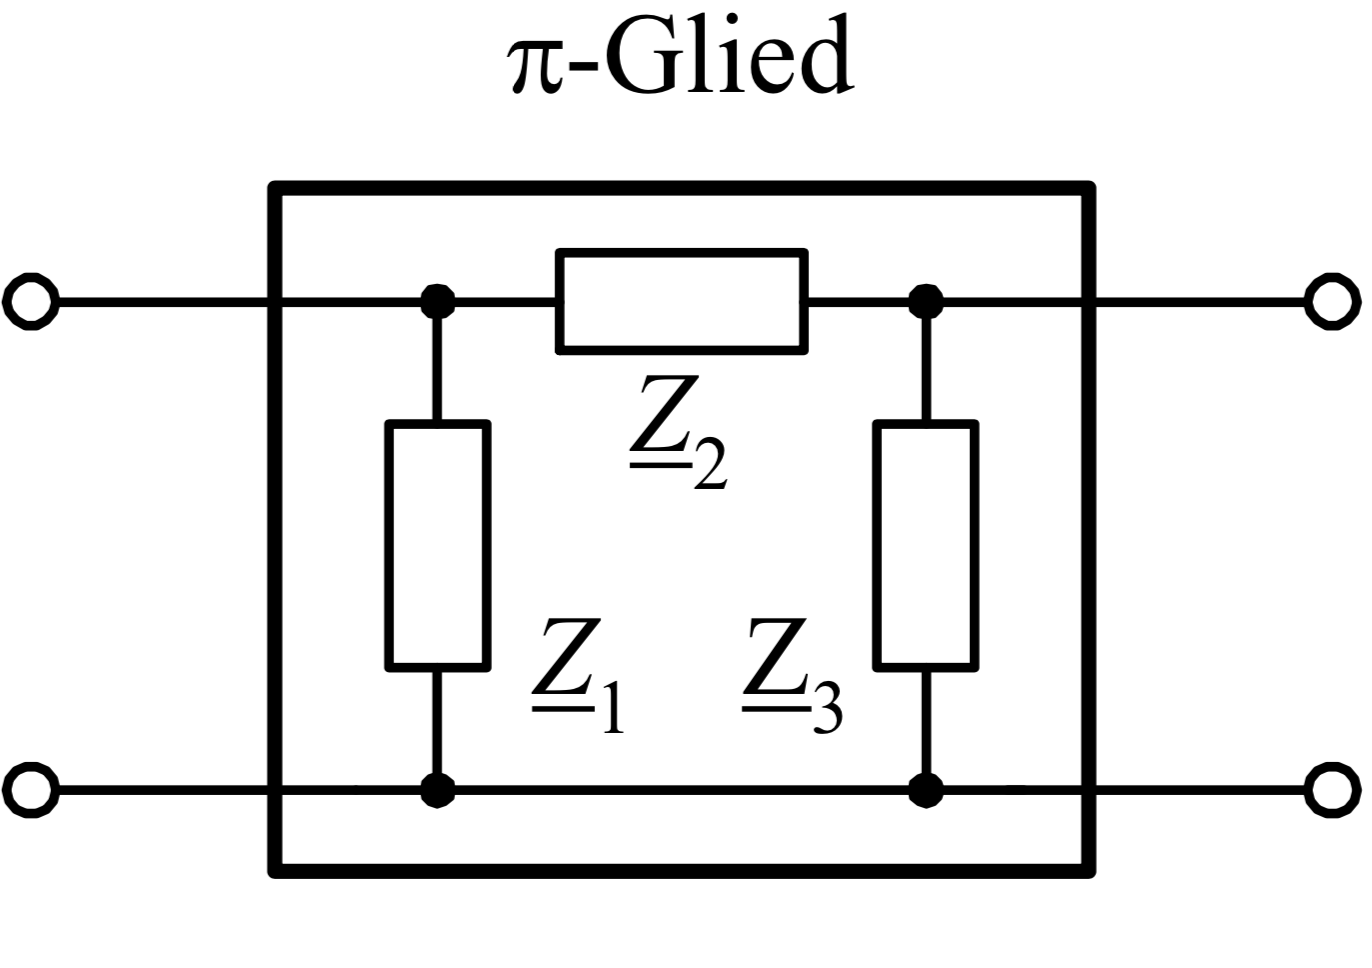
\includegraphics[width = 3cm]{pi_impedance.png}
		\label{fig:piImpedance}
		\caption{Pi-Glied \cite{2torTabelle}}
	\end{minipage}
	\begin{minipage}[h]{0.45\linewidth}
		\begin{equation}\label{equ:piImpedance}
			A_\pi = \left[\begin{matrix}
			1+\frac{\underline{Z}_2}{\underline{Z}_3}&\underline{Z}_2\\
			\frac{1}{\underline{Z}_1}+\frac{1}{\underline{Z}_3}+\frac{\underline{Z}_2}{\underline{Z}_1\underline{Z}_3}&1+\frac{\underline{Z}_2}				{\underline{Z}_1}
			\end{matrix}\right]
		\end{equation}
	\end{minipage}
\end{figure}

Wenn die ABCD-Matrix einer Schaltung gebildet wurde, kann diese direkt in die Streuparameter umgewandelt werden. Der $s_{21}$ Parameter kann wie in Formel \ref{equ:s21} beschrieben, durch einsetzten der ABCD-Matrix bestimmt werden. Für den Widerstand $R_w$ muss die verwendete Bezugsimpedanz eingesetzt werden.
\begin{equation}\label{equ:s21}
s_{21} = \frac{2}{A_{11}+\frac{A{12}}{R_w}+A_{21}*R_w+A_{22}}
\end{equation}
Die Indexierung der ABCD-Matrix wird in Abbildung \ref{equ:A_index} gezeigt
\begin{equation}\label{equ:A_index}
	A = \left[\begin{matrix}
	A_{11}&A_{12}\\A_{21}&A_{22}
	\end{matrix}\right]
\end{equation}
\newpage
